\documentclass[11pt,t]{beamer}
\usetheme{metropolis}
\metroset{progressbar=frametitle,numbering=fraction}
\usefonttheme[onlymath]{serif} % serif math: proper primes, hats and italics
\usepackage{bm}
\usepackage{amsmath,amssymb,amsfonts}
\usepackage{mathrsfs}
\usepackage{booktabs}
\usepackage{multirow}
\usepackage{graphicx}
\usepackage{xcolor}
\usepackage{tikz}
\usetikzlibrary{calc,positioning,decorations.pathmorphing,arrows.meta}
\setbeamercolor{block title}{use=normal text, fg=normal text.fg,bg=normal text.bg!80!fg}
\graphicspath{{./figures/}{./logo/}}

%%%%%%%%%%%%% Macros %%%%%%%%%%%%%
\newcommand{\rmi}{\mathrm{i}}
\newcommand{\rmd}{\mathrm{d}}
\newcommand{\DM}{\mathrm{DM}}

\title{Generative Modeling toward\\ Critical Behaviors}
\subtitle{}

\date{September 7, 2026}
\author{Yang-yang Tan}
\titlegraphic{%
  \begin{tikzpicture}[remember picture, overlay]
    % Top-left: workshop name
    \node[anchor=north west, inner sep=0pt, font=\normalsize\bfseries, text=burgundy]
      at ([xshift=0.6cm,yshift=-0.5cm]current page.north west)
      {Bridging ML and statistical field theory, ECT* Trento};
    % Bottom-right: UTokyo + IPI (aligned with author/date)
    \node[anchor=south east, inner sep=0pt] (utokyo) at ([xshift=-0.6cm,yshift=4.5cm]current page.south east) {%
      \raisebox{-0.5\height}{\includegraphics[height=3em]{UTokyo_Logotype_A_Color_RGB20240401.png}}%
      \hspace{0.4em}\rule[-0.9em]{0.4pt}{2em}\hspace{0.4em}%
      \raisebox{-0.5\height}{\includegraphics[height=2.3em]{ipilogo.png}}%
    };
    % Below UTokyo/IPI: RIKEN + iTHEMS (no separator)
    \node[anchor=north east, inner sep=0pt] at ([yshift=-0.5em]utokyo.south east) {%
      \raisebox{-0.5\height}{\includegraphics[height=2em]{logo_riken.pdf}}%
      \hspace{0.6em}%
      \raisebox{-0.5\height}{\includegraphics[height=2em]{logo_dark.pdf}}%
    };
  \end{tikzpicture}%
}

\definecolor{burgundy}{RGB}{127, 0, 32}
\definecolor{Kleinblue}{RGB}{0, 47, 167}
\newcommand{\running}[1]{\textcolor{burgundy}{#1}}
\newcommand{\kb}[1]{{\bfseries\color{Kleinblue} #1}}
% references pinned to the bottom of the page, independent of the frame content
\makeatletter
\newcommand{\refs}[1]{%
  \begin{tikzpicture}[remember picture, overlay]
    \node[anchor=south west, inner sep=0pt, align=flush left,
          text width=\dimexpr\textwidth-1.4cm\relax]
      at ([xshift=\beamer@leftmargin, yshift=0.6cm]current page.south west)
      {\raggedright\tiny\color{black!65} #1\par};
  \end{tikzpicture}}
\makeatother
\newcommand{\rtag}[1]{\textcolor{burgundy}{\textbf{#1}}}

\tikzset{
  stage/.style={
    rectangle, rounded corners=3pt,
    draw=#1!80, fill=#1!12, line width=0.8pt,
    minimum width=2.8cm, minimum height=1.7cm,
    align=center, font=\small\bfseries, text=#1!50!black,
    inner sep=4pt
  },
  tlarrow/.style={
    ->, >=stealth, line width=1.4pt, draw=gray!55,
    shorten >=2pt, shorten <=2pt
  }
}

\begin{document}
\begin{frame}[plain,noframenumbering,t]
  \inserttitlegraphic\par
  \vspace*{0.5cm}
  {\LARGE\bfseries \inserttitle\par}
  \vspace{0.4em}
  {\color{orange}\rule{\textwidth}{0.4pt}\par}
  \vspace{1.4em}
  {\normalsize\bfseries \insertauthor\par}
  \vspace{0.6em}
  {\small IPI, The University of Tokyo\par}
  \vspace{0.4em}
  {\small with \textbf{Gert Aarts}, \textbf{Diaa E.\ Habibi}, \textbf{Jinyang Li}, \textbf{Biagio Lucini} and \textbf{Lingxiao Wang}\par}
  \vspace{0.3em}
  {\normalsize \insertdate\par}
\end{frame}

% ---------------------------------------------------------------- 0
% dmqft_members.pdf: the collage region cropped from figures/dmqft.pdf (Lingxiao Wang's ERG2026 slide 2)
\begin{frame}{The DM-QFT collaboration}
  \vspace{-0.1em}
  \centerline{\includegraphics[width=1.17\textwidth]{dmqft_members}}
  \vspace{0.2em}
  \begin{columns}[T,onlytextwidth]
    \begin{column}{0.48\textwidth}
      \scriptsize\raggedright
      \kb{Board}\\[0.2em]
      \begin{tabular}{@{}l@{\hspace{0.7em}}l@{}}
        RIKEN & Lingxiao Wang\\
        Swansea & Gert Aarts\\
        SJTU & Wei Wang\\
        TU Wien & Andreas Ipp\\
        Heidelberg & Jan M.\ Pawlowski\\
        QMUL & Biagio Lucini\\
        CUHK Shenzhen & Kai Zhou
      \end{tabular}
    \end{column}
    \begin{column}{0.50\textwidth}
      \scriptsize\raggedright
      \kb{Research}\\[0.2em]
      \kb{Physics of diffusion models}\quad stochastic quantization, statistics of diffusion\\[0.2em]
      \kb{Lattice simulations}\quad 2D/3D scalars, U(1)/SU($N$) gauge fields, critical sampling\\[0.2em]
      \kb{Physics-informed kernel methods}
    \end{column}
  \end{columns}
\end{frame}

% ================================================================ Part I
% ---------------------------------------------------------------- 1
\begin{frame}{Critical phenomena across physics}
  \begin{columns}[T,onlytextwidth]
    \begin{column}{0.42\textwidth}
      \centering
      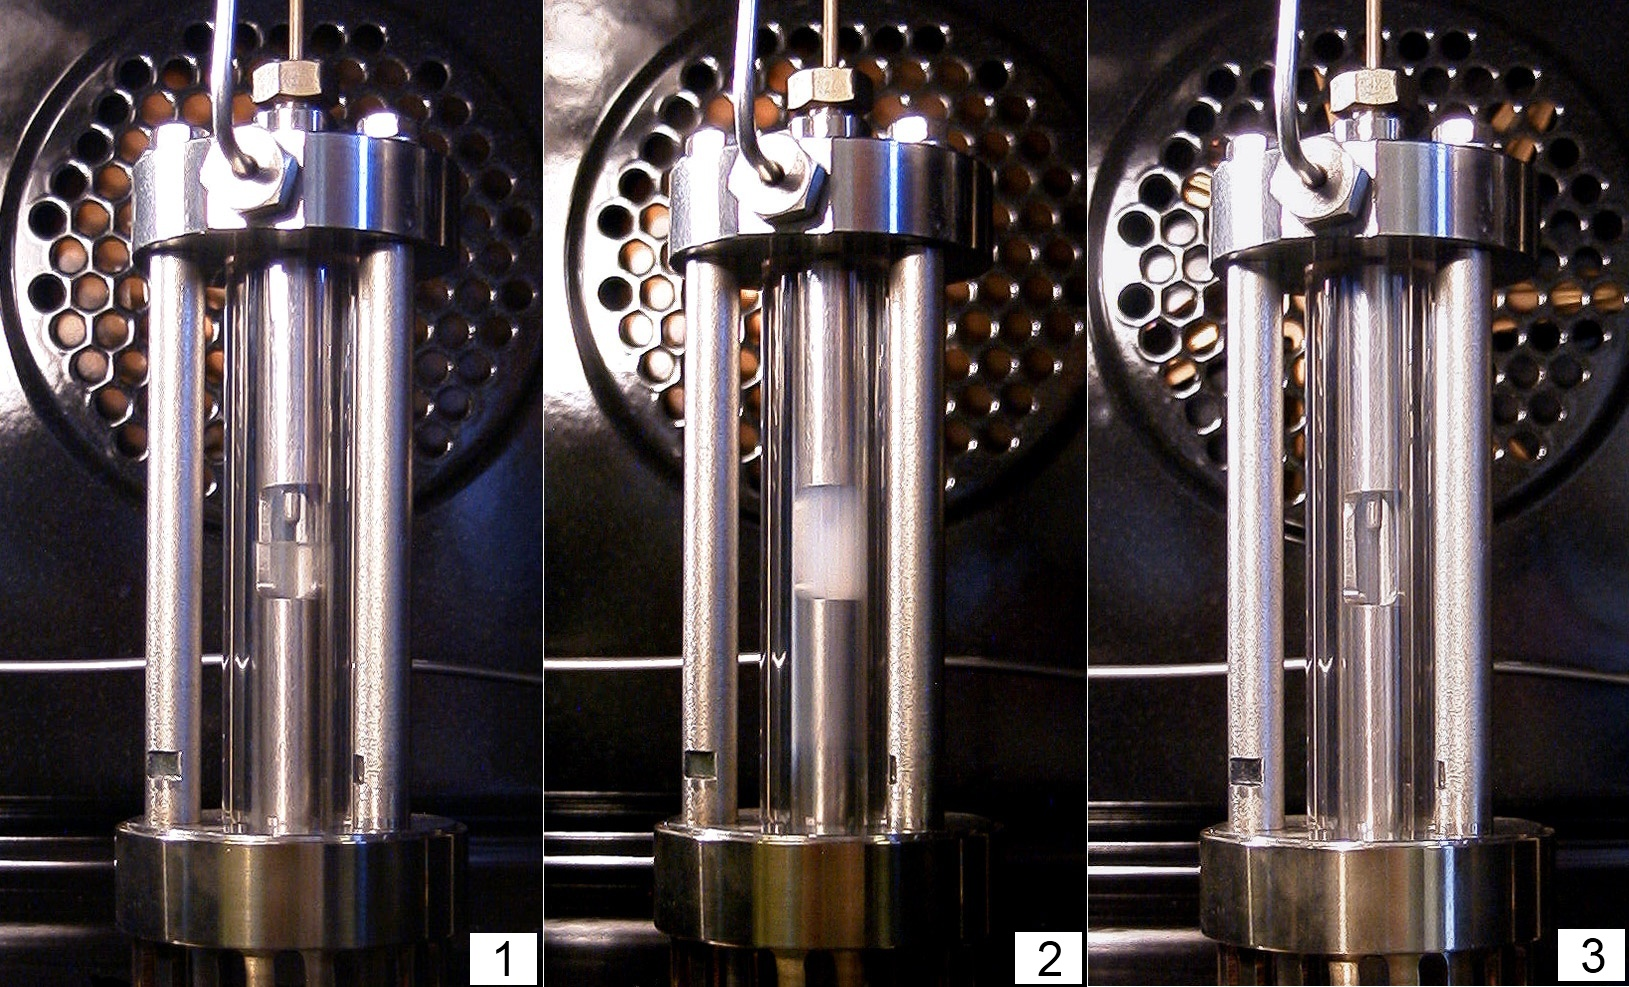
\includegraphics[height=2.35cm]{critical_opalescence_ethane.jpg}\\[0.1em]
      {\scriptsize ethane: opalescent at $T_c$}
    \end{column}
    \begin{column}{0.22\textwidth}
      \centering
      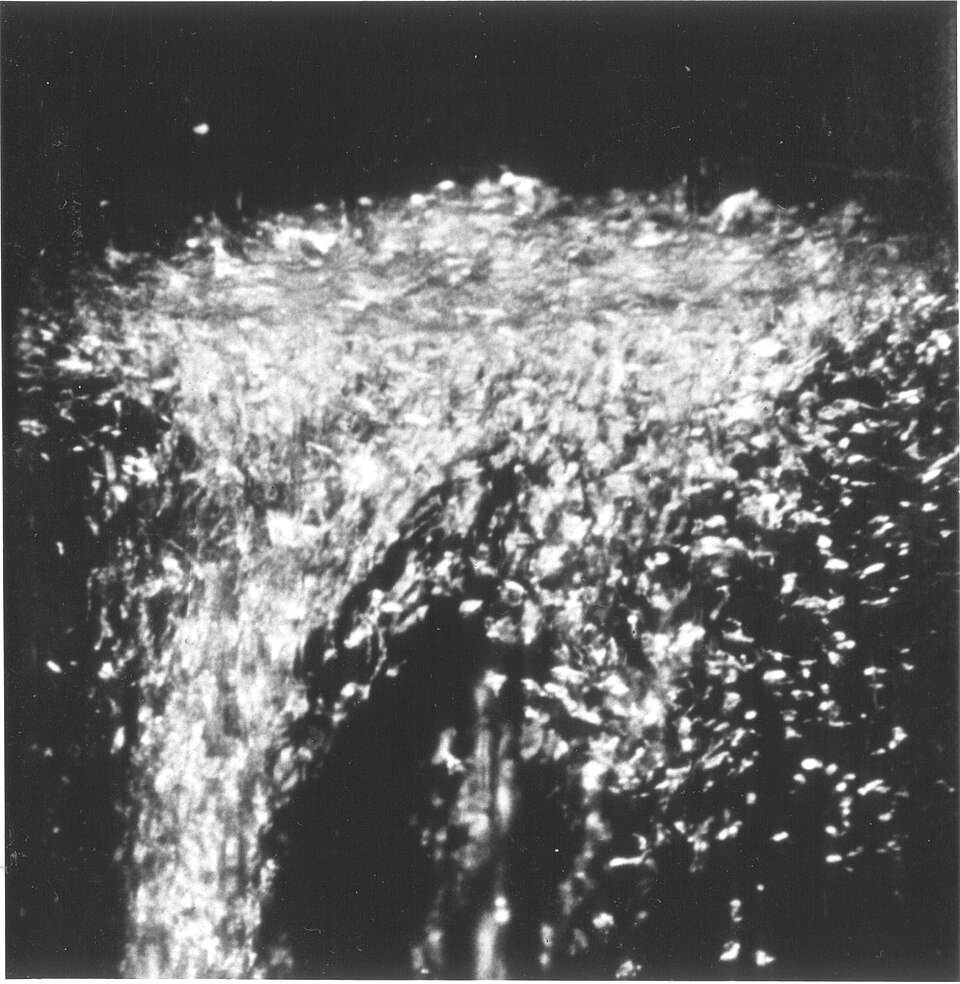
\includegraphics[height=2.35cm]{helium_lambda_point.jpg}\\[0.1em]
      {\scriptsize $^4$He at $T_\lambda$}
    \end{column}
    \begin{column}{0.33\textwidth}
      \centering
      \includegraphics[height=2.35cm]{helium_lambda_cp.png}\\[0.1em]
      {\scriptsize specific heat of $^4$He}
    \end{column}
  \end{columns}
  \vspace{1.1em}
  \begin{columns}[T,onlytextwidth]
    \begin{column}{0.40\textwidth}
      \centering
      \includegraphics[height=2.35cm]{qcd_phase_diagram_bhalerao.png}\\[0.1em]
      {\scriptsize QCD: critical end point}
    \end{column}
    \begin{column}{0.56\textwidth}
      \footnotesize\raggedright
      \kb{The same signature every time}\\[0.2em]
      no characteristic length, $\xi\to\infty$\\
      fluctuations on every scale\\
      response diverges as a power law\\
      $\chi\sim|T-T_c|^{-\gamma}$, $\xi\sim|T-T_c|^{-\nu}$\\
      \alert{exponents, not $T_c$, carry the physics}
    \end{column}
  \end{columns}
  \refs{%
    \rtag{Ethane:} S.\ Horstmann, Wikimedia Commons.\quad
    \rtag{Helium:} A.\ Leitner (1963).\quad
    \rtag{QCD phase diagram:} R.\ S.\ Bhalerao, doi:10.5170/CERN-2014-001.219.\quad
    \rtag{QCD critical point:} Stephanov, Rajagopal, Shuryak, PRL 81, 4816 (1998).}
\end{frame}

% ---------------------------------------------------------------- 2
\begin{frame}{Universality: different systems, the same numbers}
  \begin{columns}[T,onlytextwidth]
    \begin{column}{0.46\textwidth}
      \centering
      \includegraphics[width=\linewidth]{coexistence_universality.pdf}\\[-0.1em]
      {\scriptsize eight fluids, one coexistence curve}
    \end{column}
    \begin{column}{0.52\textwidth}
      \centering
      {\scriptsize
      \renewcommand{\arraystretch}{1.05}
      \setlength{\tabcolsep}{3pt}
      \begin{tabular}{lccc}
        \toprule
        & $\beta$ & $\gamma$ & $\nu$ \\
        \midrule
        fluids & $0.32$--$0.33$ & $1.23$--$1.25$ & $0.62$--$0.63$ \\
        mixtures & $0.32$--$0.33$ & $1.23$--$1.25$ & $0.62$--$0.64$ \\
        magnets & $0.32$--$0.33$ & $1.24$--$1.25$ & $0.62$--$0.64$ \\
        \alert{3D Ising} & $0.3265$ & $1.2372$ & $0.6301$ \\
        \bottomrule
      \end{tabular}}

      \vspace{0.9em}
      \footnotesize\raggedright
      \kb{Only $d$ and symmetry matter}\\[0.2em]
      fluids, mixtures, uniaxial magnets\\
      and the QCD critical end point:\\
      \alert{all 3D Ising}\\
      superfluid $^4$He: 3D XY, same story

      \vspace{0.5em}
      \kb{One model for all of them}
    \end{column}
  \end{columns}
  \refs{%
    \rtag{Coexistence curves:} Guggenheim, J.\ Chem.\ Phys.\ 13, 253 (1945); data from the NIST Chemistry WebBook, line $\rho_\pm/\rho_c=1+\tfrac34(1-T/T_c)\pm\tfrac74(1-T/T_c)^{1/3}$.\quad
    \rtag{Exponents:} Pelissetto, Vicari, Phys.\ Rept.\ 368, 549 (2002).}
\end{frame}

% ---------------------------------------------------------------- 3
\begin{frame}{Dynamic universality}
  \centering
  % 四列在 8pt 下宽 337pt，超出 307pt 文字宽；7pt 刚好放下（300pt）
  {\fontsize{7}{8.5}\selectfont
  \renewcommand{\arraystretch}{1.05}
  \setlength{\tabcolsep}{3pt}
  \begin{tabular}{llll}
    \toprule
    & conservation laws & examples & $z$ \\
    \midrule
    Model A & nonconserved $\phi$ & magnets, order--disorder alloys & $\simeq2.0$ \\
    Model B & conserved $\phi$ & alloys, diffusive mixtures & $4-\eta$ \\
    Model G & nonconserved $\phi$ $+$ conserved charges & antiferromagnets, chiral transition & $d/2$ \\
    Model H & conserved $\phi$ $+$ conserved momentum & fluids, binary liquids, QCD end point & $\simeq3.0$ \\
    \bottomrule
  \end{tabular}}
  \vspace{0.7em}
  \begin{columns}[c,onlytextwidth]
    \begin{column}{0.44\textwidth}
      \centering
      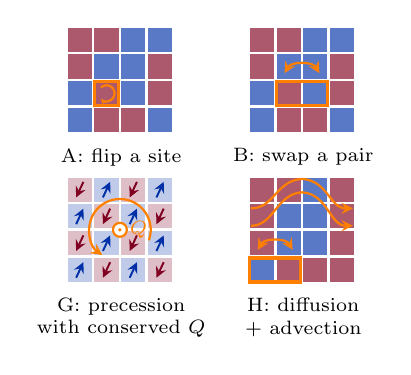
\begin{tikzpicture}[x=0.34cm,y=0.34cm,>=stealth]
        % A, B, H share the scalar +-phi pattern; G is a staggered vector spin pattern
        \foreach \dx/\dy/\lab in {0/0/{A: flip a site},6.8/0/{B: swap a pair}} {
          \begin{scope}[shift={(\dx,\dy)}]
            \foreach \i/\j/\c in {0/0/Kleinblue,1/0/burgundy,2/0/burgundy,3/0/Kleinblue,
                                  0/1/Kleinblue,1/1/burgundy,2/1/Kleinblue,3/1/burgundy,
                                  0/2/burgundy,1/2/Kleinblue,2/2/Kleinblue,3/2/burgundy,
                                  0/3/burgundy,1/3/burgundy,2/3/Kleinblue,3/3/Kleinblue}
              \fill[\c!65] (\i,\j) rectangle ++(0.9,0.9);
            \node[font=\scriptsize,anchor=north] at (2,-0.25) {\lab};
          \end{scope}}
        \draw[very thick,orange] (1,1) rectangle ++(0.9,0.9);
        \draw[-{Stealth[length=2pt,width=2pt]},thick,orange] (1.45,1.45) ++(135:0.3) arc (135:-135:0.3);
        \begin{scope}[shift={(6.8,0)}]
          \draw[very thick,orange] (1,1) rectangle ++(1.9,0.9);
          \draw[<->,thick,orange] (1.3,2.2) to[bend left=60] (2.6,2.2);
        \end{scope}
        \begin{scope}[shift={(0,-5.6)}]
          \foreach \i/\j/\c/\a in {0/0/Kleinblue/65,1/0/burgundy/245,2/0/Kleinblue/65,3/0/burgundy/245,
                                   0/1/burgundy/245,1/1/Kleinblue/65,2/1/burgundy/245,3/1/Kleinblue/65,
                                   0/2/Kleinblue/65,1/2/burgundy/245,2/2/Kleinblue/65,3/2/burgundy/245,
                                   0/3/burgundy/245,1/3/Kleinblue/65,2/3/burgundy/245,3/3/Kleinblue/65} {
            \fill[\c!25] (\i,\j) rectangle ++(0.9,0.9);
            \draw[->,\c,line width=0.7pt] (\i+0.45,\j+0.45) ++(\a+180:0.32) -- ++(\a:0.64);}
          % conserved charge Q (uniform magnetization) points out of the page (odot) and is the rotation axis
          \draw[->,thick,orange] (1.95,1.95) ++(-20:1.15) arc (-20:235:1.15);
          \fill[white] (1.95,1.95) circle (0.26);
          \draw[thick,orange] (1.95,1.95) circle (0.26);
          \fill[orange] (1.95,1.95) circle (0.07);
          \node[font=\scriptsize,orange,anchor=west,inner sep=1pt] at (2.2,1.95) {$Q$};
          \node[font=\scriptsize,anchor=north,align=center] at (2,-0.25) {G: precession\\with conserved $Q$};
        \end{scope}
        % H: a droplet in the matrix; the flow it excites goes around it and carries it
        \begin{scope}[shift={(6.8,-5.6)}]
          \foreach \i/\j/\c in {0/0/Kleinblue,1/0/burgundy,2/0/burgundy,3/0/burgundy,
                                0/1/burgundy,1/1/Kleinblue,2/1/Kleinblue,3/1/burgundy,
                                0/2/burgundy,1/2/Kleinblue,2/2/Kleinblue,3/2/burgundy,
                                0/3/burgundy,1/3/burgundy,2/3/Kleinblue,3/3/burgundy}
            \fill[\c!65] (\i,\j) rectangle ++(0.9,0.9);
          % Kawasaki swap at the interface keeps sum(phi) fixed; the flow passes over the droplet
          \draw[very thick,orange] (0,0) rectangle ++(1.9,0.9);
          \draw[<->,thick,orange] (0.3,1.2) to[bend left=60] (1.6,1.2);
          \draw[->,thick,orange] (0.05,2.1) .. controls (0.9,2.1) and (1.0,3.3) .. (1.95,3.35)
                                 .. controls (2.9,3.3) and (3.0,2.1) .. (3.85,2.1);
          \draw[->,thick,orange] (0.05,2.75) .. controls (0.9,2.75) and (1.0,3.8) .. (1.95,3.85)
                                 .. controls (2.9,3.8) and (3.0,2.75) .. (3.85,2.75);
          \node[font=\scriptsize,anchor=north,align=center] at (2,-0.25) {H: diffusion\\$+$ advection};
        \end{scope}
      \end{tikzpicture}
    \end{column}
    \begin{column}{0.54\textwidth}
      \small\raggedright
      \kb{Same statics, different dynamics}\\[0.3em]
      the equilibrium weight $e^{-S}$ is identical\\[0.2em]
      relaxation time $\tau\sim\xi^{z}$, $\omega(k)\sim k^{z}$\\[0.2em]
      conservation laws and mode couplings determine $z$\\[0.4em]
      \alert{this talk: Model B}\\
      \alert{conserved $\phi$, $z=4-\eta$}
    \end{column}
  \end{columns}
  \refs{%
    \rtag{Classification:} Hohenberg, Halperin, Rev.\ Mod.\ Phys.\ 49, 435 (1977).\quad
    \rtag{Model B exponent:} Halperin, Hohenberg, Ma, PRB 10, 139 (1974).\quad
    \rtag{Model G and chiral QCD:} Rajagopal, Wilczek, Nucl.\ Phys.\ B 399, 395 (1993).\quad
    \rtag{Model H and QCD:} Son, Stephanov, PRD 70, 056001 (2004).}
\end{frame}

% ---------------------------------------------------------------- 4
\begin{frame}{Sampling near criticality: a data-driven route}
  \footnotesize\raggedright
  \vspace{-0.4em}
  \kb{Lattice $\phi^4$}\ \ $S[\phi]=\sum_x\big[-2\kappa\sum_{\mu}\phi_x\phi_{x+\hat\mu}+\phi_x^2+\lambda(\phi_x^2-1)^2\big]$, Ising class
  \vspace{0.1em}
  \begin{columns}[T,onlytextwidth]
    \begin{column}{0.52\textwidth}
      \footnotesize\raggedright
      \kb{Why Monte Carlo struggles}\\[0.1em]
      the physics sits in the infrared\\
      local moves: $\tau\sim L^{z}$, \alert{Anna's talk}\\
      cluster moves: special models only\\
      needed: independent configurations
    \end{column}
    \begin{column}{0.46\textwidth}
      \footnotesize\raggedright
      \kb{Learn the distribution from data}\\[0.1em]
      input: configurations, \alert{not $S[\phi]$}\\
      output: independent new samples\\
      critical physics reproduced?
    \end{column}
  \end{columns}
  \vspace{0.1em}
  \centering
  \uncover<2->{%
  \begin{tikzpicture}[font=\scriptsize,>=stealth]
    \foreach \t/\i in {0/0,0.01/1,0.03/2,0.08/3,1/4}
      \node[inner sep=0pt] (p\i) at (1.3*\i,0) {\includegraphics[width=0.9cm]{phi4_diffuse_t\t.png}};
    \draw[->,thick,burgundy] ([yshift=0.1cm]p0.north west) -- ([yshift=0.1cm]p4.north east)
      node[midway,above] {add noise until the configuration is forgotten};
    \draw[<-,thick,Kleinblue] ([yshift=-0.1cm]p0.south west) -- ([yshift=-0.1cm]p4.south east)
      node[midway,below] {a learned drift removes the noise again: a new configuration};
  \end{tikzpicture}}
  \vspace{-0.3em}

  \begin{uncoverenv}<3->
  {\footnotesize\raggedright
  \kb{This talk}\ \ \alert{statics}: sampling across the transition, unseen $L$\ \ \alert{dynamics}: Model B\\[0.1em]
  \kb{Also here}\ \ flows: \alert{Gurtej's talk}\ \ PIKs: \alert{Jan's, Friederike's, Renzo's talks}\par}
  \end{uncoverenv}
  \refs{%
    \rtag{Cluster updates:} Swendsen, Wang, PRL 58, 86 (1987); Wolff, PRL 62, 361 (1989).\quad
    \rtag{Flows:} Albergo, Kanwar, Shanahan, PRD 100, 034515 (2019).\quad
    \rtag{Physics-informed kernels:} Ihssen, Kapust, Pawlowski, arXiv:2510.26678.\quad
    \rtag{Diffusion models on the lattice:} Wang, Aarts, Zhou, JHEP 05, 060 (2024); Aarts et al., MLST 6, 025004 (2025); Zhu et al., JHEP 03, 111 (2026).\quad
    \rtag{Critical slowing down in DMs:} Del Bono et al., arXiv:2605.12597.}
\end{frame}

% ---------------------------------------------------------------- 5
\begin{frame}{Score-based diffusion is learned stochastic quantization}
  \small
  \kb{Forward VE process}\quad $\Sigma(1)\gtrsim$ data spread, so $p_{t=1}$ is a broad Gaussian
  \vspace{-0.3em}
  \begin{equation*}
    \rmd\phi=\sigma^{t}\,\rmd w,\qquad
    \phi_t=\phi_0+\Sigma(t)\,\eta,\qquad
    \Sigma^2(t)=\frac{\sigma^{2t}-1}{2\ln\sigma}
  \end{equation*}
  \vspace{-0.9em}

  \kb{Reverse SDE and ODE}\quad same marginals $p_t$; Euler--Maruyama sampler
  \vspace{-0.3em}
  \begin{equation*}
    \rmd\phi=-g^2(t)\,s_\theta(\phi,t)\,\rmd t+g(t)\,\rmd\bar w,\qquad
    \frac{\rmd\phi}{\rmd t}=-\tfrac12 g^2(t)\,s_\theta(\phi,t)
  \end{equation*}
  \vspace{-1.0em}

  \onslide<2->
  \kb{Score matching}\quad minimizer $s=\nabla_\phi\log p_t$; samples only, \alert{never $S[\phi]$}
  \vspace{-0.3em}
  \begin{equation*}
    \mathcal L(\theta)=\Big\langle\big\|\Sigma(t)\,s_\theta\big(\phi_0+\Sigma(t)\eta,\,t\big)+\eta\big\|^2\Big\rangle_{t,\phi_0,\eta}
  \end{equation*}
  \vspace{-1.0em}

  \onslide<3->
  \kb{Small-time limit}\quad the drift of stochastic quantization: \alert{is it reproduced?}
  \vspace{-0.3em}
  \begin{equation*}
    s_\theta(\phi,t\to0)\ \to\ \nabla_\phi\log p_{\rm data}=-\nabla_\phi S[\phi]
  \end{equation*}
  \refs{%
    \rtag{Score SDE:} Song et al., ICLR (2021).\quad
    \rtag{DSM:} Vincent, Neural Comput.\ 23, 1661 (2011).\quad
    \rtag{Stochastic quantization:} Parisi, Wu, Sci.\ Sin.\ 24, 483 (1981).\quad
    \rtag{DM as stochastic quantization:} Wang, Aarts, Zhou, JHEP 05, 060 (2024); Fukushima, Kamata, Hirono, JPSJ 94, 031010 (2025).}
\end{frame}

% ---------------------------------------------------------------- 6
\begin{frame}{Score network and reference configurations}
  \centering
  \includegraphics[width=0.6\textwidth]{architecture_ncsnpp_v2}
  \vspace{0.1em}
  % left column: the physics (put in by hand vs learned); right column: how it is realised
  \begin{columns}[T,onlytextwidth]
    \begin{column}{0.48\textwidth}
      \footnotesize\raggedright
      \kb{Physics built in}\\[0.1em]
      periodic lattice: circular padding\\
      translation symmetry: convolutions\\
      \alert{nothing else}, not even $\phi\to-\phi$\\
      gauge equivariance: \alert{Thomas's talk}
    \end{column}
    \begin{column}{0.50\textwidth}
      \footnotesize\raggedright
      \kb{Architecture}\\[0.1em]
      U-Net, $L\to L/8$: reaches the infrared\\
      skip connections keep the ultraviolet\\
      no dense layer: any $L$, same weights\\
      diffusion as an RG flow: \alert{Yuto's talk}
    \end{column}
  \end{columns}
  % [T] columns pull their content up by 1ex, so the skip must be larger than it looks
  \vspace{0.7em}
  \begin{uncoverenv}<2->
  \begin{columns}[T,onlytextwidth]
    \begin{column}{0.48\textwidth}
      \footnotesize\raggedright
      \kb{Physics learned}\\[0.1em]
      the action $S[\phi]$, never given\\
      the $\phi\to-\phi$ symmetry\\
      \quad\alert{Satoshi and Jinyang's talk}\\
      critical correlations, which phase
    \end{column}
    \begin{column}{0.50\textwidth}
      \footnotesize\raggedright
      \kb{Reference configurations}\\[0.1em]
      HMC with Wolff reflections\\
      $\kappa$ below, at and above $\kappa_c$\\
      $10240$ / $2560$ configs, \alert{all it ever sees}\\
      data-free: \alert{Biagio's, Shinichi's talks}
    \end{column}
  \end{columns}
  \end{uncoverenv}
  \refs{%
    \rtag{NCSN++:} Song et al., ICLR (2021).\quad
    The noise level $t$ enters every Res Block through an embedding, panel (b).\quad
    $\kappa_c=0.27088$ (2D, $L=128$), $0.19225$ (3D, $L=64$) from Binder crossings; 3D: Hasenbusch, J.\ Phys.\ A 32, 4851 (1999).}
\end{frame}

% ---------------------------------------------------------------- 7
\begin{frame}{Magnetization and action density}
  \centering
  \includegraphics[width=0.88\textwidth]{mS_joint_3panels}\\[0.1em]
  {\scriptsize 2D, $L=128$: joint distribution $P(\bar\phi,s)$ of mean field and action density}
  \vspace{0.5em}
  \begin{columns}[T,onlytextwidth]
    \begin{column}{0.28\textwidth}
      \centering
      \kb{Symmetric}\\[0.3em]
      \footnotesize one peak at $\bar\phi=0$\\
      contours coincide
    \end{column}
    \begin{column}{0.34\textwidth}
      \centering
      \kb{Critical}\\[0.3em]
      \footnotesize two finite-volume peaks\\
      shape and $\chi$ agree
    \end{column}
    \begin{column}{0.38\textwidth}
      \centering
      \kb{Broken}\\[0.3em]
      \footnotesize peaks at the right $\pm v$\\
      \alert{too wide}: $\chi$ $30\%$ too large
    \end{column}
  \end{columns}
  \vspace{0.6em}
  {\footnotesize all three phases right, one defect: the ordered peak is too wide\par}
  \refs{%
    \rtag{Cumulants in diffusion models:} Aarts, Habibi, Wang, Zhou, MLST 6, 025004 (2025).\quad
    $\chi=V(\langle\bar\phi^2\rangle-\langle|\bar\phi|\rangle^2)$; contours enclose $20/50/90/98\%$ of the probability mass.}
\end{frame}

% ---------------------------------------------------------------- 8
\begin{frame}{The propagator converges with training}
  \begin{columns}[T,onlytextwidth]
    \begin{column}{0.33\textwidth}
      \footnotesize\raggedright
      \kb{Resolve the scales}\\[0.1em]
      $G(k)=\langle|\tilde\phi(k)|^2\rangle$\\
      one number per $k$,\\
      the loss averages them

      \vspace{0.5em}
      \onslide<2->
      \kb{2D, critical}\\[0.1em]
      short distances first\\
      the infrared last

      \vspace{0.5em}
      \kb{3D, critical}\\[0.1em]
      early overshoot at all $k$\\
      infrared settles first

      \vspace{0.5em}
      \kb{After training}\\[0.1em]
      \alert{all six couplings}\\
      match HMC at every $k$
    \end{column}
    \begin{column}{0.65\textwidth}
      \centering
      \onslide<1->
      \includegraphics[width=\linewidth]{2D_kappa=0.2705_prop.pdf}\\[0.2em]
      \includegraphics[width=\linewidth]{3D_kappa=0.1923_prop.pdf}
    \end{column}
  \end{columns}
  \refs{%
    Left panels log--log, right panels log--linear, zero mode excluded. Each curve is one checkpoint of the same training run, sampled with the reverse SDE.}
\end{frame}

% ---------------------------------------------------------------- 9
\begin{frame}{Anomalous dimension at the critical point}
  \begin{columns}[T,onlytextwidth]
    \begin{column}{0.46\textwidth}
      \centering
      \includegraphics[width=\linewidth]{prop_k=0.2705_log_log.pdf}\\[0.1em]
      {\scriptsize 2D, $L=128$, $\kappa=0.2705$, $\eta=1/4$}
    \end{column}
    \begin{column}{0.46\textwidth}
      \centering
      \includegraphics[width=\linewidth]{prop_k=0.1923_log_log.pdf}\\[0.1em]
      {\scriptsize 3D, $L=64$, $\kappa=0.1923$, $\eta\simeq0.036$}
    \end{column}
  \end{columns}
  \vspace{0.8em}
  \begin{columns}[T,onlytextwidth]
    \begin{column}{0.31\textwidth}
      \centering
      \kb{Critical scaling}\\[0.3em]
      \footnotesize $G(k)\propto k^{-(2-\eta)}$\\
      $\eta=0$ for a free field
    \end{column}
    \begin{column}{0.31\textwidth}
      \centering
      \onslide<2->
      \kb{2D Ising}\\[0.3em]
      \footnotesize \alert{$\eta=1/4$ resolved}\\
      off the free $1/k^2$
    \end{column}
    \begin{column}{0.31\textwidth}
      \centering
      \onslide<2->
      \kb{3D Ising}\\[0.3em]
      \footnotesize $\eta\simeq0.036$, lines close\\
      DM and HMC coincide
    \end{column}
  \end{columns}
  \vspace{1.0em}
  \begin{uncoverenv}<2->
  {\centering\footnotesize the interacting fixed point leaves its fingerprint in $\eta$, and the samples carry it\par}
  \end{uncoverenv}
  \refs{%
    \rtag{Exponents:} Pelissetto, Vicari, Phys.\ Rept.\ 368, 549 (2002); Hasenbusch, J.\ Phys.\ A 32, 4851 (1999).\quad
    Converged models, trained and sampled at the same $L$.}
\end{frame}

% ---------------------------------------------------------------- 10
\begin{frame}{Diagnostic 1: is the learned drift the force $-\nabla S$?}
  \centering
  \includegraphics[width=0.98\textwidth]{score_quality_vs_epoch_L128_3panel_ema}\\[0.2em]
  {\scriptsize $s_\theta(\phi,t\to0)$ against $-\nabla S[\phi]$: direction, overall error, magnitude}
  \vspace{0.6em}
  \begin{columns}[T,onlytextwidth]
    \begin{column}{0.36\textwidth}
      \footnotesize\raggedright
      \kb{The test}\\[0.2em]
      $s_\theta(\phi,t\to0)$ vs.\ $-\nabla S[\phi]$\\
      on HMC configurations\\
      no $S$ during training
    \end{column}
    \begin{column}{0.31\textwidth}
      \footnotesize\raggedright
      \onslide<2->
      \kb{Direction first}\\[0.2em]
      cosine $0.9\to0.998$\\
      within $\sim10^2$ epochs\\
      same in every phase
    \end{column}
    \begin{column}{0.31\textwidth}
      \footnotesize\raggedright
      \onslide<3->
      \kb{Magnitude later}\\[0.2em]
      $3$--$4\times$ too strong\\
      $\to1$ by $5\times10^3$ epochs\\
      \alert{$-\nabla S$ reconstructed}\\
      from samples alone
    \end{column}
  \end{columns}
  \refs{%
    2D, $L=128$; the same trends in 3D. The test isolates the network as a function: errors that build up along the reverse trajectory are not seen here.}
\end{frame}

% ---------------------------------------------------------------- 11
\begin{frame}{Diagnostic 2: a Metropolis test of the learned drift}
  \begin{columns}[T,onlytextwidth]
    \begin{column}{0.56\textwidth}
      \small
      \kb{One step with the learned drift}
      \vspace{-0.4em}
      \begin{equation*}
        \psi=\phi+h\,s_\theta(\phi,t\to0)+\sqrt{2h}\,\eta
      \end{equation*}
      \vspace{-1.3em}
      \begin{equation*}
        \alpha=\frac{p(\psi)\,q(\phi\,|\,\psi)}{p(\phi)\,q(\psi\,|\,\phi)},\qquad p\propto e^{-S}
      \end{equation*}
      \vspace{-0.8em}

      \onslide<2->
      \kb{What it measures}\\
      $e^{-S}$ judges the proposal\\
      near one: the local drift is right\\
      no reverse trajectory involved

      \vspace{0.35em}
      \onslide<3->
      \kb{Result}\\
      \alert{above $65\%$ at every $L\ge8$, every $\kappa$}\\
      $0.85$--$0.91$ on the largest lattices
    \end{column}
    \begin{column}{0.42\textwidth}
      \centering
      \onslide<3->
      \includegraphics[width=0.78\linewidth]{acceptance_vs_epoch_L128_multi_kappa_ema}\\[-0.1em]
      \includegraphics[width=0.78\linewidth]{acceptance_vs_epoch_3d_L64_multi_kappa_ema}
    \end{column}
  \end{columns}
  \refs{%
    \rtag{MALA scaling:} Roberts, Rosenthal, J.\ R.\ Statist.\ Soc.\ B 60, 255 (1998).\quad
    \rtag{Metropolis-adjusted diffusion:} Lam et al., arXiv:2605.09654; Zhu et al., JHEP 03, 111 (2026).\quad
    Step size $h\propto L^{-d}$, chosen where early and late checkpoints differ most.}
\end{frame}

% ---------------------------------------------------------------- 12
\begin{frame}{Diagnostic 3: what is a DM sample worth?}
  \begin{columns}[T,onlytextwidth]
    \begin{column}{0.43\textwidth}
      \footnotesize\raggedright
      \kb{Why not autocorrelations}\\[0.1em]
      DM samples are independent,\\
      $\tau_{\rm int}=\tfrac12$ even when biased

      \vspace{0.4em}
      \kb{Error-matched sample size}
      \vspace{-0.5em}
      \begin{equation*}
        N_{{\rm eff},O}=\frac{\sigma_{p,O}^2}{\delta_O^2+{\rm Var}(\bar O_{\DM})}
      \end{equation*}
      \vspace{-0.9em}

      exact samples with the same\\
      total error, bias $\delta_O$ included

      \vspace{0.4em}
      \kb{Bias from the HMC reference}\\[0.1em]
      $\delta_O$: difference of the means\\
      one $N_{\rm eff}$ per observable

      \vspace{0.4em}
      \kb{Another probe}\\[0.1em]
      a configurational thermometer:\\
      \alert{Diaa's talk}
    \end{column}
    \begin{column}{0.55\textwidth}
      \centering
      \onslide<2->
      \includegraphics[width=\linewidth]{ess_mse_vs_epoch_L128_k0.2705_sigma450_ema}\\[0.1em]
      {\scriptsize 2D, $L=128$, critical: $N_{\rm eff}/N_{\DM}$ along training}

      \vspace{0.6em}
      \small\raggedright
      \kb{Early}: bias dominated, ratios $\ll1$\\[0.2em]
      \kb{Late}: \alert{ratios close to one} for scalars\\
      and for the propagator at all scales\\[0.2em]
      \kb{3D critical}: all but $S/V$ reach one,\\
      the action bias remains
    \end{column}
  \end{columns}
  \refs{%
    Propagator bands: modes averaged over the infrared, intermediate and ultraviolet ranges. Errors from bootstrap; the HMC reference variance includes its autocorrelation.}
\end{frame}

% ---------------------------------------------------------------- 13
\begin{frame}{Train on small lattices, sample a lattice never seen}
  \begin{columns}[T,onlytextwidth]
    \begin{column}{0.40\textwidth}
      \centering
      \includegraphics[width=\linewidth]{L64_crossL_3d_k0.1923_multiL_loglog}\\[0.1em]
      {\scriptsize multi-$L$ training $\to L=64$}
    \end{column}
    \begin{column}{0.40\textwidth}
      \centering
      \includegraphics[width=\linewidth]{L64_crossL_3d_k0.1923_singleL_loglog}\\[0.1em]
      {\scriptsize single-$L$ baselines $\to L=64$}
    \end{column}
  \end{columns}
  \vspace{0.6em}
  \begin{uncoverenv}<2->
  \begin{columns}[T,onlytextwidth]
    \begin{column}{0.56\textwidth}
      \footnotesize\raggedright
      \kb{3D, $\kappa=0.1923$: $L_{\rm train}\le32\ \Longrightarrow\ L=64$}\\[0.1em]
      $\{4,8,16,32\}$ tracks HMC \alert{down to $k_{\min}$}\\
      $\{4,8\}$ misses the infrared rise\\
      single $L$: $32$ closest, $4$ fails\\
      several volumes teach the infrared
    \end{column}
    \begin{column}{0.42\textwidth}
      \centering
      {\scriptsize
      \renewcommand{\arraystretch}{0.95}
      \setlength{\tabcolsep}{5pt}
      \begin{tabular}{lc}
        \toprule
        training $L$ & acceptance \\
        \midrule
        $\{4,8\}$ & $0.578(8)$ \\
        $\{4,8,16\}$ & $0.830(6)$ \\
        $\{4,8,16,32\}$ & $0.877(6)$ \\
        $\{64\}$, in distribution & $0.911(9)$ \\
        \bottomrule
      \end{tabular}}
    \end{column}
  \end{columns}
  \end{uncoverenv}
  \refs{%
    \rtag{Multi-lattice generative models:} M\'at\'e, Fleuret, MLST 5, 045053 (2024); Bauer, Kapust, Pawlowski, Temmen, SciPost Phys.\ 19, 077 (2025); Singha et al., ICLR (2025); Zhu et al., JHEP 03, 111 (2026).\quad
    \rtag{Cost of large-volume training:} Abbott et al., EPJA 59, 257 (2023).\quad
    No $L=64$ information enters training or sampling.}
\end{frame}

% ---------------------------------------------------------------- 14
\begin{frame}{Unseen lattice: symmetric and broken phases}
  \begin{columns}[T,onlytextwidth]
    \begin{column}{0.48\textwidth}
      \centering
      \includegraphics[width=0.80\linewidth]{L64_crossL_3d_k0.18_multiL_loglog}
    \end{column}
    \begin{column}{0.48\textwidth}
      \centering
      \includegraphics[width=0.80\linewidth]{L64_crossL_3d_k0.2_multiL_loglog}
    \end{column}
  \end{columns}
  \vspace{0.4em}
  \begin{columns}[T,onlytextwidth]
    \begin{column}{0.48\textwidth}
      \footnotesize\raggedright
      \kb{Symmetric phase, $\kappa=0.18$}\\[0.1em]
      $\xi$ is a few spacings, so every\\
      training lattice sees all of it\\
      $\{4,8\}$ undershoots $k_{\min}$ by $15\%$\\
      $\{4,8,16\}$ and up: on top of HMC
    \end{column}
    \begin{column}{0.48\textwidth}
      \footnotesize\raggedright
      \kb{Broken phase, $\kappa=0.2$}\\[0.1em]
      condensate, not $\xi$, sets the infrared\\
      $L=4,8$ still flip sign: no ordered\\
      lattice in the set, $\{4,8\}$ invents\\
      \alert{$4\times$ too much infrared power}\\
      $\{4,8,16\}$ and up: on top of HMC
    \end{column}
  \end{columns}
  \vspace{0.6em}
  {\footnotesize\raggedright
   \kb{Rule of thumb}\quad largest training lattice within $2\times$ of the target\\
   $k_{\min}=2\pi/64$ is below every training momentum, $k=0$ is not shown\par}
  \refs{3D, $\lambda=0.9$, $L=64$, same training sets as on the previous slide.}
\end{frame}

% ---------------------------------------------------------------- 15
\begin{frame}{Zero mode at the unseen size, and an exact refinement}
  \centering
  {\scriptsize
  \renewcommand{\arraystretch}{0.95}
  \setlength{\tabcolsep}{5pt}
  \begin{tabular}{lcccc}
    \toprule
    3D, $L=64$, $\kappa=0.1923\simeq\kappa_c$ & $\langle|\bar\phi|\rangle$ & $\chi$ & $\langle S\rangle/V$ & $U_L$ \\
    \midrule
    HMC & $0.1165(9)$ & $621(15)$ & $-0.11671(5)$ & $0.516(4)$ \\
    DM trained at $L=64$ & $0.147(2)$ & $755(49)$ & $-0.0975(3)$ & $0.559(7)$ \\
    DM $\{4,8\}$ & $0.0287(9)$ & $94(5)$ & $-0.10747(5)$ & $0.24(3)$ \\
    DM $\{4,8,16\}$ & $0.064(2)$ & $445(22)$ & $-0.1180(1)$ & $0.28(2)$ \\
    DM $\{4,8,16,32\}$ & $0.100(2)$ & $694(30)$ & $-0.1125(1)$ & $0.44(1)$ \\
    DM $\{4,8,16,32\}$ $+$ MC, learned drift & $0.126(2)$ & $678(26)$ & $-0.1175(1)$ & $0.528(7)$ \\
    DM $\{4,8,16,32\}$ $+$ MC, true $-\nabla S$ & \alert{$0.116(2)$} & \alert{$642(23)$} & \alert{$-0.1165(1)$} & \alert{$0.509(7)$} \\
    \bottomrule
  \end{tabular}}
  \vspace{0.8em}
  \begin{columns}[T,onlytextwidth]
    \begin{column}{0.49\textwidth}
      \footnotesize\raggedright
      \kb{Multi-$L$ beats training at $L=64$}\\[0.1em]
      $\chi$, $\langle S\rangle/V$, $\langle|\bar\phi|\rangle$ closer to HMC\\
      infrared learned from four sizes\\
      \alert{holds up to $2\times$ the largest training $L$}
    \end{column}
    \begin{column}{0.49\textwidth}
      \footnotesize\raggedright
      \kb{DM samples seed an exact chain}\\[0.1em]
      Metropolis with the learned drift\\
      $+$ cluster moves, exact for $e^{-S}$\\
      learned drift: the zero mode stalls\\
      true force $-\nabla S$: HMC recovered
    \end{column}
  \end{columns}
  \refs{%
    \rtag{Embedded cluster:} Brower, Tamayo, PRL 62, 1087 (1989).\quad
    Same chain length for both drifts. DM rows use the field range of the HMC reference; without it the $\chi$ of the $L=64$ model doubles, the multi-$L$ one barely moves.}
\end{frame}

% ================================================================ Part II
% ---------------------------------------------------------------- 16
\begin{frame}{From statics to dynamics: learn one transition kernel}
  \small
  \kb{So far}\quad the score of $e^{-S}$: static ensembles, no physical time\\[0.2em]
  \kb{Now}\quad autonomous stochastic dynamics $\partial_t\phi=\mathcal F[\phi,\xi]$, Markov, no time origin

  \vspace{0.5em}
  \onslide<2->
  \kb{Transformation kernel}\quad no explicit $t$ dependence; its law is $p_{\Delta t}(\phi'\,|\,\phi)$
  \vspace{-0.3em}
  \begin{equation*}
    \Delta\phi(t)
    \equiv\phi(t+\Delta t)-\phi(t)
    =\mathcal T_{\Delta t}[\phi(t),w]
    \equiv\int_t^{t+\Delta t}\!\rmd\tau\,
    \mathcal F[\phi(\tau),\xi(\tau;w)]
  \end{equation*}
  \vspace{-0.6em}

  \onslide<3->
  \kb{Exact composition}
  \begin{center}
    $\begin{aligned}
    \phi_{j+1}
    &=\phi_j+\mathcal T_{\Delta t}[\phi_j,w_j],
    &&j=0,\ldots,n-1,\\
    \phi_0&=\phi(t),
    &\phi_n&=\phi(t+n\Delta t).
    \end{aligned}$\\[0.5em]
    Chapman--Kolmogorov: \alert{one interval fixes every multiple of $\Delta t$},\\ in and out of equilibrium
  \end{center}
  \refs{%
    Pairs $(\phi_t,\phi_{t+\Delta t})$ are direct samples of the kernel, from a simulation or an experiment.
    Colored noise: enlarge the state, $X=(\phi,\eta)$, and the joint kernel composes again.}
\end{frame}

% ---------------------------------------------------------------- 17
\begin{frame}{Conditional diffusion draws one step}
  \begin{columns}[T,onlytextwidth]
    \begin{column}{0.53\textwidth}
      \centering
      \includegraphics[width=\linewidth]{schematic}\\[0.3em]
      {\normalsize $\Delta\phi\sim p_\theta(\,\cdot\mid\phi_t)$
      \qquad
      $\phi_{t+\Delta t}=\phi_t+\Delta\phi$}
    \end{column}
    \begin{column}{0.45\textwidth}
      \footnotesize\raggedright
      \kb{Condition}\\[0.1em]
      present field $\phi_t$ as a clean input

      \vspace{0.35em}
      \kb{Target}\\[0.1em]
      the increment $\Delta\phi$, diffused\\
      and denoised as in Part I

      \vspace{0.35em}
      \kb{Physics learned}\\[0.1em]
      $p(\Delta\phi\,|\,\phi_t)$ from pairs alone\\
      \alert{no drift, noise or free energy}

      \vspace{0.35em}
      \kb{Physics built in}\\[0.1em]
      $\sum_x\Delta\phi_x=0$ by projection\\
      at every step, $M$ conserved exactly
    \end{column}
  \end{columns}
  \refs{%
    \rtag{Fast ODE solver:} Zheng et al., DPM-Solver-v3, NeurIPS (2023).\quad
    Same U-Net as in Part I with $\phi_t$ as a second input channel; one kernel step costs a few dozen network calls.}
\end{frame}

% ---------------------------------------------------------------- 18
\begin{frame}{Model B: conserved dynamics}
  \begin{center}
    2D conserved $\phi^4$ field
  \end{center}
  \begin{columns}[c]
    \begin{column}{0.66\textwidth}
      \begin{align*}
        \partial_t\phi(\bm{x},t)
        &=\Gamma\nabla^2\frac{\delta F[\phi]}{\delta\phi(\bm{x},t)}
          +\zeta(\bm{x},t),\\
        \langle\zeta(\bm{x},t)\zeta(\bm{x}',t')\rangle
        &=-2T\Gamma\nabla^2\delta^{(d)}(\bm{x}-\bm{x}')\delta(t-t'),\\
        F[\phi]
        &=\int d^dx\left[\tfrac{1}{2}(\nabla\phi)^2
        +\tfrac{r}{2}\phi^2+\tfrac{u}{4}\phi^4\right].
      \end{align*}
    \end{column}
    \begin{column}{0.32\textwidth}
      \centering
      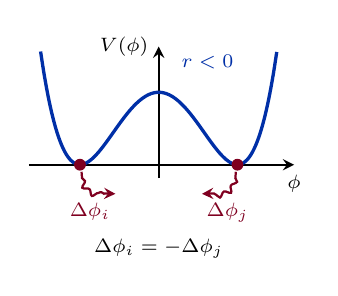
\begin{tikzpicture}[font=\scriptsize,>=stealth]
        \draw[->,thick] (-1.65,0.25) -- (1.72,0.25) node[below] {$\phi$};
        \draw[->,thick] (0,0.08) -- (0,1.75) node[left] {$V(\phi)$};
        \draw[very thick,Kleinblue,domain=-1.5:1.5,samples=80,smooth]
          plot (\x,{0.25+0.92*(\x*\x-1)^2});
        \node[Kleinblue] at (0.62,1.55) {$r<0$};
        \fill[burgundy] (-1,0.25) circle (0.075);
        \fill[burgundy] (1,0.25) circle (0.075);
        \draw[->,burgundy,thick,decorate,
              decoration={snake,amplitude=0.3mm,segment length=1.4mm,
                          pre length=0.8mm,post length=1.5mm}]
          (-0.98,0.16) .. controls (-0.98,-0.08) and (-0.84,-0.12) .. (-0.55,-0.12)
          node[midway,below=1pt] {$\Delta\phi_i$};
        \draw[->,burgundy,thick,decorate,
              decoration={snake,amplitude=0.3mm,segment length=1.4mm,
                          pre length=0.8mm,post length=1.5mm}]
          (0.98,0.16) .. controls (0.98,-0.08) and (0.84,-0.12) .. (0.55,-0.12)
          node[midway,below=1pt] {$\Delta\phi_j$};
        \node at (0,-0.82) {$\Delta\phi_i=-\Delta\phi_j$};
      \end{tikzpicture}
    \end{column}
  \end{columns}
  % align 在 minipage 末尾会丢掉 belowdisplayskip，没有这行下一栏会压到公式
  \vspace{0.6em}
  \begin{uncoverenv}<2->
  \begin{columns}[T,onlytextwidth]
    \begin{column}{0.42\textwidth}
      \centering
      \kb{Conserved mean}\\[0.4em]
      $M(t)\equiv V^{-1}\!\int d^dx\,\phi(\bm{x},t)$\\[0.3em]
      $M(t)=M(0)$
    \end{column}
    \begin{column}{0.30\textwidth}
      \centering
      \kb{Critical dynamics}\\[0.4em]
      $\tau\propto \xi^z\propto k^{-z}$\\[0.3em]
      $z=4-\eta$
    \end{column}
    \begin{column}{0.26\textwidth}
      \centering
      \kb{Kernel interval}\\[0.4em]
      $\Delta t=10$\\[0.3em]
      $\gg$ a solver step
    \end{column}
  \end{columns}
  \vspace{0.6em}
  {\centering\footnotesize
    $-\Gamma\nabla^2$ is a physics-informed kernel: \alert{Jan's and Renzo's talks}\par}
  \end{uncoverenv}
  \refs{%
    \rtag{Model B:} Hohenberg, Halperin, Rev.\ Mod.\ Phys.\ 49, 435 (1977).\quad
    Reference trajectories from a direct stochastic integrator (SOSRA) of these equations, on the lattice action of Part I.\quad
    \rtag{Kernel:} $-\Gamma\nabla^2$ in front of $\delta F/\delta\phi$ leaves the equilibrium $e^{-F/T}$ unchanged and sets the dynamics.}
\end{frame}

% ---------------------------------------------------------------- 19
% pair_*.png: one sample of each recipe below, evolved with SOSRA over Δt=10,
% colour scale RdBu ±1.6 (coarsening, L=64, ℓ=8, w=1.5, A=1.3, η=0.2) and ±2.2 (critical, L=32, Z=0.7, m²=0.2, M=0.4)
\newcommand{\pairpanel}[1]{\raisebox{-.5\height}{\includegraphics[width=1.0cm]{#1}}}
\begin{frame}{What the kernel is trained on}
  \footnotesize\raggedright
  \vspace{-0.2em}
  \begin{columns}[T,onlytextwidth]
    \begin{column}{0.47\textwidth}
      \footnotesize\raggedright
      \kb{Critical kernel}\quad $\kappa=\kappa_c$, $L=32$\\[0.2em]
      Gaussian field $\chi$ with propagator
      \vspace{-0.4em}
      \begin{equation*}
        \langle\chi_k\,\chi_{-k}\rangle=\frac{1}{Zk^2+m^2},\quad \phi_0=M+\chi
      \end{equation*}
      \vspace{-0.9em}

      $Z$ sets the amplitude, $m^2$ the correlation length, $M$ the mean, all random over a broad range

      \vspace{1.0em}
      \centerline{%
        \begin{tabular}{@{}c@{\hspace{1pt}}c@{\hspace{1pt}}c@{\hspace{1pt}}c@{\hspace{1pt}}c@{}}
          \pairpanel{pair_crit_chi} & $\scriptstyle\rightarrow$ &
          \pairpanel{pair_crit_phi0} & $\scriptstyle\rightarrow$ &
          \pairpanel{pair_crit_phi1}\\[0.1em]
          \scriptsize $\chi$ & & \scriptsize $\phi_0=M+\chi$ & & \scriptsize $\phi_{\Delta t}$
        \end{tabular}}
    \end{column}
    \begin{column}{0.51\textwidth}
      \footnotesize\raggedright
      \onslide<2->
      \kb{Coarsening kernel}\quad $\kappa=0.85$, $L\le64$\\[0.2em]
      $g$ Gaussian with $\langle g(\bm{x})\,g(0)\rangle=e^{-\bm{x}^2/2\ell^2}$
      \vspace{-0.4em}
      \begin{equation*}
        \phi_0=A\tanh\!\big(\tfrac{\ell}{w}\,g\big)+\eta\,\xi
      \end{equation*}
      \vspace{-0.9em}

      domains $\pm A$ of size $\ell$, walls of width $w$, white noise $\xi$ of level $\eta$\\
      $\ell$, $w$, $A$, $\eta$ random over a broad range

      \vspace{1.0em}
      \centerline{%
        \begin{tabular}{@{}c@{\hspace{1pt}}c@{\hspace{1pt}}c@{\hspace{1pt}}c@{\hspace{1pt}}c@{\hspace{1pt}}c@{\hspace{1pt}}c@{}}
          \pairpanel{pair_cg_g} & $\scriptstyle\rightarrow$ &
          \pairpanel{pair_cg_tanh} & $\scriptstyle\rightarrow$ &
          \pairpanel{pair_cg_phi0} & $\scriptstyle\rightarrow$ &
          \pairpanel{pair_cg_phi1}\\[0.1em]
          \scriptsize $g$ & & \scriptsize $A\tanh(\tfrac{\ell}{w}g)$ & & \scriptsize $\phi_0$ & & \scriptsize $\phi_{\Delta t}$
        \end{tabular}}
    \end{column}
  \end{columns}
  \vspace{0.1em}
  \begin{uncoverenv}<2->
  \kb{Target}\quad Model B (SOSRA) run from $\phi_0$ over $\Delta t=10$, $\Delta\phi=\phi_{\Delta t}-\phi_0$\\[0.2em]
  \kb{The point}\quad the kernel learns the rule of motion, not trajectories\\
  \alert{every test is an extrapolation}: other ensembles, longer times, larger lattices
  \end{uncoverenv}
  \refs{%
    $Z$ log-uniform in $[0.05,10]$, $m^2\in[0,0.8]$, $M\in[-0.9,0.9]$; $\ell$ log-uniform in $[2,L/3]$, $w\in[0.7,3]$, $A\in[0.8,1.8]$, $\eta\in[0.05,0.35]$, $1/8$ pure noise; $51200$ pairs per $L$.}
\end{frame}

% ---------------------------------------------------------------- 20
\begin{frame}{Equilibrium and nonequilibrium evolution}
  \begin{columns}[T]
    \begin{column}{0.30\textwidth}
      \kb{Critical point}\\
      2D, $L=32$\\
      strongly coupled

      \vspace{0.2em}
      \kb{Initial ensembles}\\
      HMC equilibrium\\
      Gaussian quench

      \vspace{0.2em}
      \kb{Composition}\\
      \alert{$\bm{200}$} kernel steps\\
      $t=2000$

      \vspace{0.2em}
      \kb{Against SOSRA}\\
      $G_1(t)$ agrees\\
      $M(t)=M(0)$
    \end{column}
    \begin{column}{0.68\textwidth}
      \centering
      \includegraphics[width=0.86\linewidth]{validation_L32}
    \end{column}
  \end{columns}
\end{frame}

% ---------------------------------------------------------------- 21
\begin{frame}{Every mode relaxes at its own rate}
  \begin{columns}[T,onlytextwidth]
    \begin{column}{0.46\textwidth}
      \footnotesize\raggedright
      \kb{Two-time correlation $\rho_n(\Delta t)$}\\[0.1em]
      mode $k_n$ at $t$ against $t+\Delta t$,\\
      on the equilibrium chain,\\
      averaged over time origins

      \vspace{0.5em}
      \onslide<2->
      \kb{Conserved dynamics is slow}\\[0.1em]
      $\tau_n\propto k_n^{-z}$ with $z\simeq4$:\\
      the softest mode outlives $n=4$\\
      by two orders of magnitude

      \vspace{0.5em}
      \onslide<3->
      \kb{Iterated kernel against SOSRA}\\[0.1em]
      lines: direct integration\\
      markers: the kernel, one step $=10$\\
      \alert{the same curve for every mode}\\
      over the whole range of lags\\
      next: read off $\tau_n$, test $\tau_n\propto k_n^{-z}$
    \end{column}
    \begin{column}{0.52\textwidth}
      \centering
      \onslide<1->
      \includegraphics[width=\linewidth]{rho_L32}\\[0.1em]
      {\scriptsize 2D, $L=32$, critical, diagonal modes $n=1$--$4$}
    \end{column}
  \end{columns}
  \refs{%
    Time origins along the $t=2000$ equilibrium chain of the previous slide. Errors: leave-one-trajectory-out jackknife.}
\end{frame}

% ---------------------------------------------------------------- 22
\begin{frame}{The critical exponent emerges}
  \begin{columns}[T]
    \begin{column}{0.44\textwidth}
      \kb{Mode autocorrelation}
      \small
      \begin{equation*}
        \rho_n(\Delta t)=
        \frac{\left\langle\operatorname{Re}\!\left[
          \phi_n(t+\Delta t)\,\phi_n^*(t)\right]\right\rangle_t}
        {\sqrt{\left\langle G_n(t+\Delta t)\right\rangle_t
               \left\langle G_n(t)\right\rangle_t}}
      \end{equation*}
      $\phi_n\equiv\phi(\bm{k}_n)$,\quad $G_n=V^{-1}\langle|\phi_n|^2\rangle$

      \kb{Dynamic scaling}
      \begin{equation*}
        \rho_n(\Delta t)=f(\Delta t/\tau_n),\qquad
        \tau_n\propto\widehat k_n^{-z}
      \end{equation*}
      all modes on one curve

      \onslide<2->
      \kb{Fits at $L=32$}

      \alert{$\bm{z_{\rm DM}=3.792(19)}$}

      \alert{$\bm{z_{\rm SOSRA}=3.764(36)}$}

      exact: $z=4-\eta=3.75$
    \end{column}
    \begin{column}{0.54\textwidth}
      \onslide<1->
      \includegraphics[width=0.94\linewidth]{collapse_dm_L32}
      {\fontsize{6}{7}\selectfont
      \textcolor{Kleinblue}{$z=4-\eta=15/4=3.75$}. \rtag{Exact.} Halperin et al., PRB 10, 139 (1974).\\
      \textcolor{Kleinblue}{$z=3.83(10),\ 3.716(17)$}. \rtag{MC.} Schweitzer et al., NPB 984, 115944 (2022).\\
      \textcolor{Kleinblue}{$z=3.95(10)$}. \rtag{Kawasaki MC.} Zheng, PLA 277, 257 (2000), erratum 282, 132 (2001).\\
      \textcolor{Kleinblue}{$z=3.79\pm0.05$}. \rtag{MC RG.} Moseley et al., J. Stat. Phys. 57, 421 (1989).\\
      \textcolor{Kleinblue}{$z=3.80$}. \rtag{MC RG.} Yalabik and Gunton, PRB 25, 534 (1982).
      \par}
    \end{column}
  \end{columns}
\end{frame}

% ---------------------------------------------------------------- 23
\begin{frame}{Beyond the exponent: the scaling function}
  \begin{columns}[T,onlytextwidth]
    \begin{column}{0.50\textwidth}
      \centering
      \includegraphics[width=\linewidth]{gamma_invx_dm_L32}\\[0.1em]
      {\scriptsize decay rate of the learned kernel's $\rho_n$, $x=\Delta t/\tau_n$}
    \end{column}
    \begin{column}{0.48\textwidth}
      \footnotesize\raggedright
      \kb{Effective decay rate}\\[0.1em]
      $\Gamma_{\rm eff}(x)=-\,d\ln\rho_n/dx$\\
      a pure exponential: a flat line

      \vspace{0.4em}
      \kb{Short times: set by the statics}\\[0.1em]
      fluctuation--dissipation relation\\
      $\Gamma_0=\widehat k_n^2/G_n$,\quad $r=\Gamma_0\tau_n\simeq1.8$

      \vspace{0.4em}
      \onslide<2->
      \kb{Long times: a slower single rate}\\[0.1em]
      $\lambda_0\simeq0.27$, seven times below $r$\\
      detailed balance: $\rho_n$ is a positive\\
      sum of exponentials, the rate can\\
      only fall, from $r$ to the gap $\lambda_0$

      \vspace{0.4em}
      \kb{All four modes on one curve}\\[0.1em]
      \alert{the whole function is reproduced},\\
      not only $z$. SOSRA has the tail too
    \end{column}
  \end{columns}
  \refs{%
    Dashed: $\lambda_0+1/(2x)$. Dash-dotted: fit $f(x)=e^{-\lambda_0x}(1+ax)^{-b}$ with the sum rule $\lambda_0+ab=r$, $b\simeq\tfrac12$. The direct SOSRA dynamics gives the same curve within errors.}
\end{frame}

% ---------------------------------------------------------------- 24
\begin{frame}{One kernel step, every mode at once}
  \centering
  \includegraphics[width=0.94\textwidth]{one_step_diagonal_combined}\\[0.1em]
  {\scriptsize $\rho_n(\Delta t)$ after one kernel step from equilibrium fields, against the lattice momentum $\widehat k$}
  \vspace{0.4em}
  \begin{columns}[T,onlytextwidth]
    \begin{column}{0.34\textwidth}
      \footnotesize\raggedright
      \kb{The kernel alone}\\[0.1em]
      no error accumulates\\
      all modes in one plot
    \end{column}
    \begin{column}{0.32\textwidth}
      \footnotesize\raggedright
      \kb{Two intervals}\\[0.1em]
      $\Delta t=0.5$: the fast modes\\
      $\Delta t=10$: the slow modes\\
      the interval is a choice
    \end{column}
    \begin{column}{0.32\textwidth}
      \footnotesize\raggedright
      \kb{Two sizes}\\[0.1em]
      kernels from $L=32$ and\\
      from $L=8,16,32$\\
      \alert{both right at $L=64$},\\
      a size neither has seen
    \end{column}
  \end{columns}
  \refs{%
    Circles SOSRA, squares the single-size kernel, triangles the multi-size kernel. Filled markers $\Delta t=0.5$, open markers $\Delta t=10$.}
\end{frame}

% ---------------------------------------------------------------- 25
\begin{frame}{Prediction on unseen $L=64$}
  \begin{columns}[T]
    \begin{column}{0.44\textwidth}
      \kb{Size extrapolation}

      \small
      \begin{center}
        $L_{\rm train}=8,16,32$\ \ {$\Longrightarrow$}\ \ \alert{$\bm{L=64}$}\\[0.3em]
        no $L=64$ trajectory ever seen
      \end{center}

      \onslide<2->
      \kb{Fits at $L=64$}

      \alert{$\bm{z_{\rm DM}=3.855(21)}$}

      \alert{$\bm{z_{\rm Model\,B}=3.867(23)}$}

      \vspace{0.6em}
      \kb{Finite-size drift}

      $L=32\to64$: $3.78\to3.86$\\
      DM and the direct integrator\\
      move together

      \vspace{0.6em}
      \kb{Cost}

      as fast as the best direct solver
    \end{column}
    \begin{column}{0.54\textwidth}
      \centering
      \onslide<1->
      \includegraphics[width=\linewidth,height=0.62\textheight,keepaspectratio]{reverse_nfe_tau_L64}
      \par\vspace{0.3em}
      {\scriptsize relaxation time of every mode at $L=64$: direct integrator, learned kernel with the reverse SDE, and with the fast ODE solver\par}
    \end{column}
  \end{columns}
\end{frame}

% ---------------------------------------------------------------- 26
\begin{frame}{Phase separation on unseen $L=128$}
  \begin{columns}[T]
    \begin{column}{0.44\textwidth}
      \kb{Sign-field correlation}
      \small
      \begin{equation*}
        \sigma(\bm{x},t)=\operatorname{sgn}\phi(\bm{x},t)
      \end{equation*}
      \begin{equation*}
        C(r,t)=\left\langle\sigma(\bm{x},t)\,\sigma(\bm{x}+\bm{r},t)\right\rangle
      \end{equation*}

      $L(t)$: first zero of $C(r,t)$

      \kb{Phase-ordering scaling}
      \begin{equation*}
        C(r,t)=g\big(r/L(t)\big)
      \end{equation*}
      \begin{equation*}
        L(t)\propto t^{1/3}
      \end{equation*}

      \kb{Size extrapolation}

      $L_{\rm train}\le64$\ \ {$\Longrightarrow$}\ \ \alert{$\bm{L=128}$}

      \alert{$\bm{L(t)\propto t^{1/3}}$}\\[0.2em]
      $L_{\rm DM}/L_{\rm SOSRA}=1$ within $2\%$
    \end{column}
    \begin{column}{0.54\textwidth}
      \centering
      \vspace*{-0.6em}
      \includegraphics[width=\linewidth,height=0.50\textheight,keepaspectratio]{collapse_dm_L128}
      \par\vspace{0.15em}
      {\raggedright
      \fontsize{5.2}{5.6}\selectfont
      \textcolor{Kleinblue}{$t^{1/3}$}. \rtag{LSW theory.} Lifshitz and Slyozov, JPCS 19, 35 (1961).\\
      \textcolor{Kleinblue}{Asymptotic $t^{1/3}$, corrections}. \rtag{Conserved Ising.} Huse, PRB 34, 7845 (1986).\\
      \textcolor{Kleinblue}{$t^{1/3}$, scaling}. \rtag{2D critical Model B.} Rogers et al., PRB 37, 9638 (1988).\\
      \textcolor{Kleinblue}{$t^{1/3}$ scaling}. \rtag{Review.} Bray, Adv. Phys. 43, 357 (1994).\\
      \textcolor{Kleinblue}{$t^{1/3}$}. \rtag{Polymer experiment.} Krausch et al., PRL 71, 3669 (1993).\\
      \textcolor{Kleinblue}{Critical $\alpha=1/3$}. \rtag{2D CH.} K\"onig et al., PCCP 23, 24823 (2021).\\
      \textcolor{Kleinblue}{$\alpha_L=0.34,0.37$ from perimeter}. \rtag{Membrane.} Zhiliakov et al., BBA 1863, 183446 (2021).\\
      \textcolor{Kleinblue}{$t^{1/3}$}. \rtag{Passive membrane, CH.} Arnold et al., PRL 131, 128402 (2023).\\
      \textcolor{Kleinblue}{$t^{1/3}$}. \rtag{HP1 Model B.} Tortora et al., PNAS 120, e2211855120 (2023).\\
      \textcolor{Kleinblue}{Long-time $t^{1/3}$}. \rtag{Diffusive polymer Model B.} Garcia et al., JCP 159, 214904 (2023).
      \par}
    \end{column}
  \end{columns}
\end{frame}

% ---------------------------------------------------------------- 27
\begin{frame}{Sharp domain walls: Porod's law}
  \begin{columns}[T,onlytextwidth]
    \begin{column}{0.48\textwidth}
      \footnotesize\raggedright
      \kb{Structure factor of the sign field}
      \vspace{-0.5em}
      \begin{equation*}
        S(k,t)=\tfrac1V\big\langle|\sigma(k,t)|^2\big\rangle
      \end{equation*}
      \vspace{-0.9em}

      the Fourier transform of $C(r,t)$

      \vspace{0.3em}
      \kb{One length again}
      \vspace{-0.5em}
      \begin{equation*}
        S(k,t)=L(t)^2\,h\big(kL(t)\big)
      \end{equation*}
      \vspace{-0.8em}

      \kb{Porod tail}\\[0.1em]
      sharp walls between domains give\\
      $h(x)\propto x^{-(d+1)}=x^{-3}$ at large $x$

      \vspace{0.4em}
      \kb{Generated fields at $L=128$}\\[0.1em]
      $t=100$--$1000$ collapse on one curve\\
      \alert{the tail follows $k^{-3}$}\\
      a size the kernel never saw
    \end{column}
    \begin{column}{0.50\textwidth}
      \centering
      \includegraphics[width=\linewidth]{sk_collapse_dm_L128}\\[0.1em]
      {\scriptsize the DM trajectory of the previous slide, rescaled by its own $L(t)$}
    \end{column}
  \end{columns}
  \refs{%
    \rtag{Porod law:} Porod, Kolloid-Z.\ 124, 83 (1951); Bray, Adv.\ Phys.\ 43, 357 (1994).\quad
    $h$ is the 2D Fourier transform of $g$. The peak near $kL(t)\simeq2$--$3$ marks the domain spacing.}
\end{frame}

% ---------------------------------------------------------------- 28
\begin{frame}[c]{Summary}
  \relax % keep beamer from reading the next brace group as a subtitle
  {\centering\large Learned scores $\longrightarrow$ critical statics and critical dynamics\par}
  \vspace{0.3em}
  \begin{columns}[T,onlytextwidth]
    \begin{column}{0.33\textwidth}
      \centering
      {\small $\phi^4$ in 2D and 3D}\\[0.4em]
      {\alert{\large all three regimes}}\\[0.3em]
      {\scriptsize $\eta$ resolved, $P(\bar\phi,s)$ right\\ bias only in the zero mode}
    \end{column}
    \begin{column}{0.33\textwidth}
      \centering
      {\small Diagnostics}\\[0.4em]
      {\alert{\large $s_\theta\to-\nabla S$}}\\[0.3em]
      {\scriptsize $-\nabla S$ from samples alone\\ Metropolis accepts it}
    \end{column}
    \begin{column}{0.33\textwidth}
      \centering
      {\small Unseen volumes}\\[0.4em]
      {\alert{\large $\{4,8,16,32\}\Rightarrow64$}}\\[0.3em]
      {\scriptsize beats training at $L=64$\\ exact refinement $\to$ HMC}
    \end{column}
  \end{columns}
  \vspace{1.1em}
  \begin{columns}[T,onlytextwidth]
    \begin{column}{0.33\textwidth}
      \centering
      {\small Transition kernel}\\[0.4em]
      {\alert{\large $z_{\rm DM}=3.792(19)$}}\\[0.3em]
      {\scriptsize exact $z=3.75$\\ pairs only, no equations}
    \end{column}
    \begin{column}{0.33\textwidth}
      \centering
      {\small Beyond training sizes}\\[0.4em]
      {\alert{\large $L=64$, $L=128$}}\\[0.3em]
      {\scriptsize $z=3.855(21)$ vs.\ $3.867(23)$\\ as fast as direct solvers}
    \end{column}
    \begin{column}{0.33\textwidth}
      \centering
      {\small Phase separation}\\[0.4em]
      {\alert{\large $L(t)\propto t^{1/3}$}}\\[0.3em]
      {\scriptsize within $2\%$ of Model B\\ collapse, Porod tail $k^{-3}$}
    \end{column}
  \end{columns}
  \vspace{0.7em}
  {\centering\small
    Outlook: noise schedules for the zero mode (EDM2, RG-inspired),\\ diffusion samples as seeds for exact MC, Model H, gauge fields\par}
  \vspace{0.4em}
  {\centering
    {\large Thank you!}\par}
\end{frame}

\end{document}
